\documentclass{standalone}
 
% Required package
\usepackage{tikz}
\usepackage{amssymb}
\usepackage{ntheorem}
\usepackage{tensor}
%\usepackage{physics}
\usepackage[italicdiff]{physics}
\usepackage{calc}
 \usetikzlibrary {backgrounds,mindmap}
\begin{document}
 
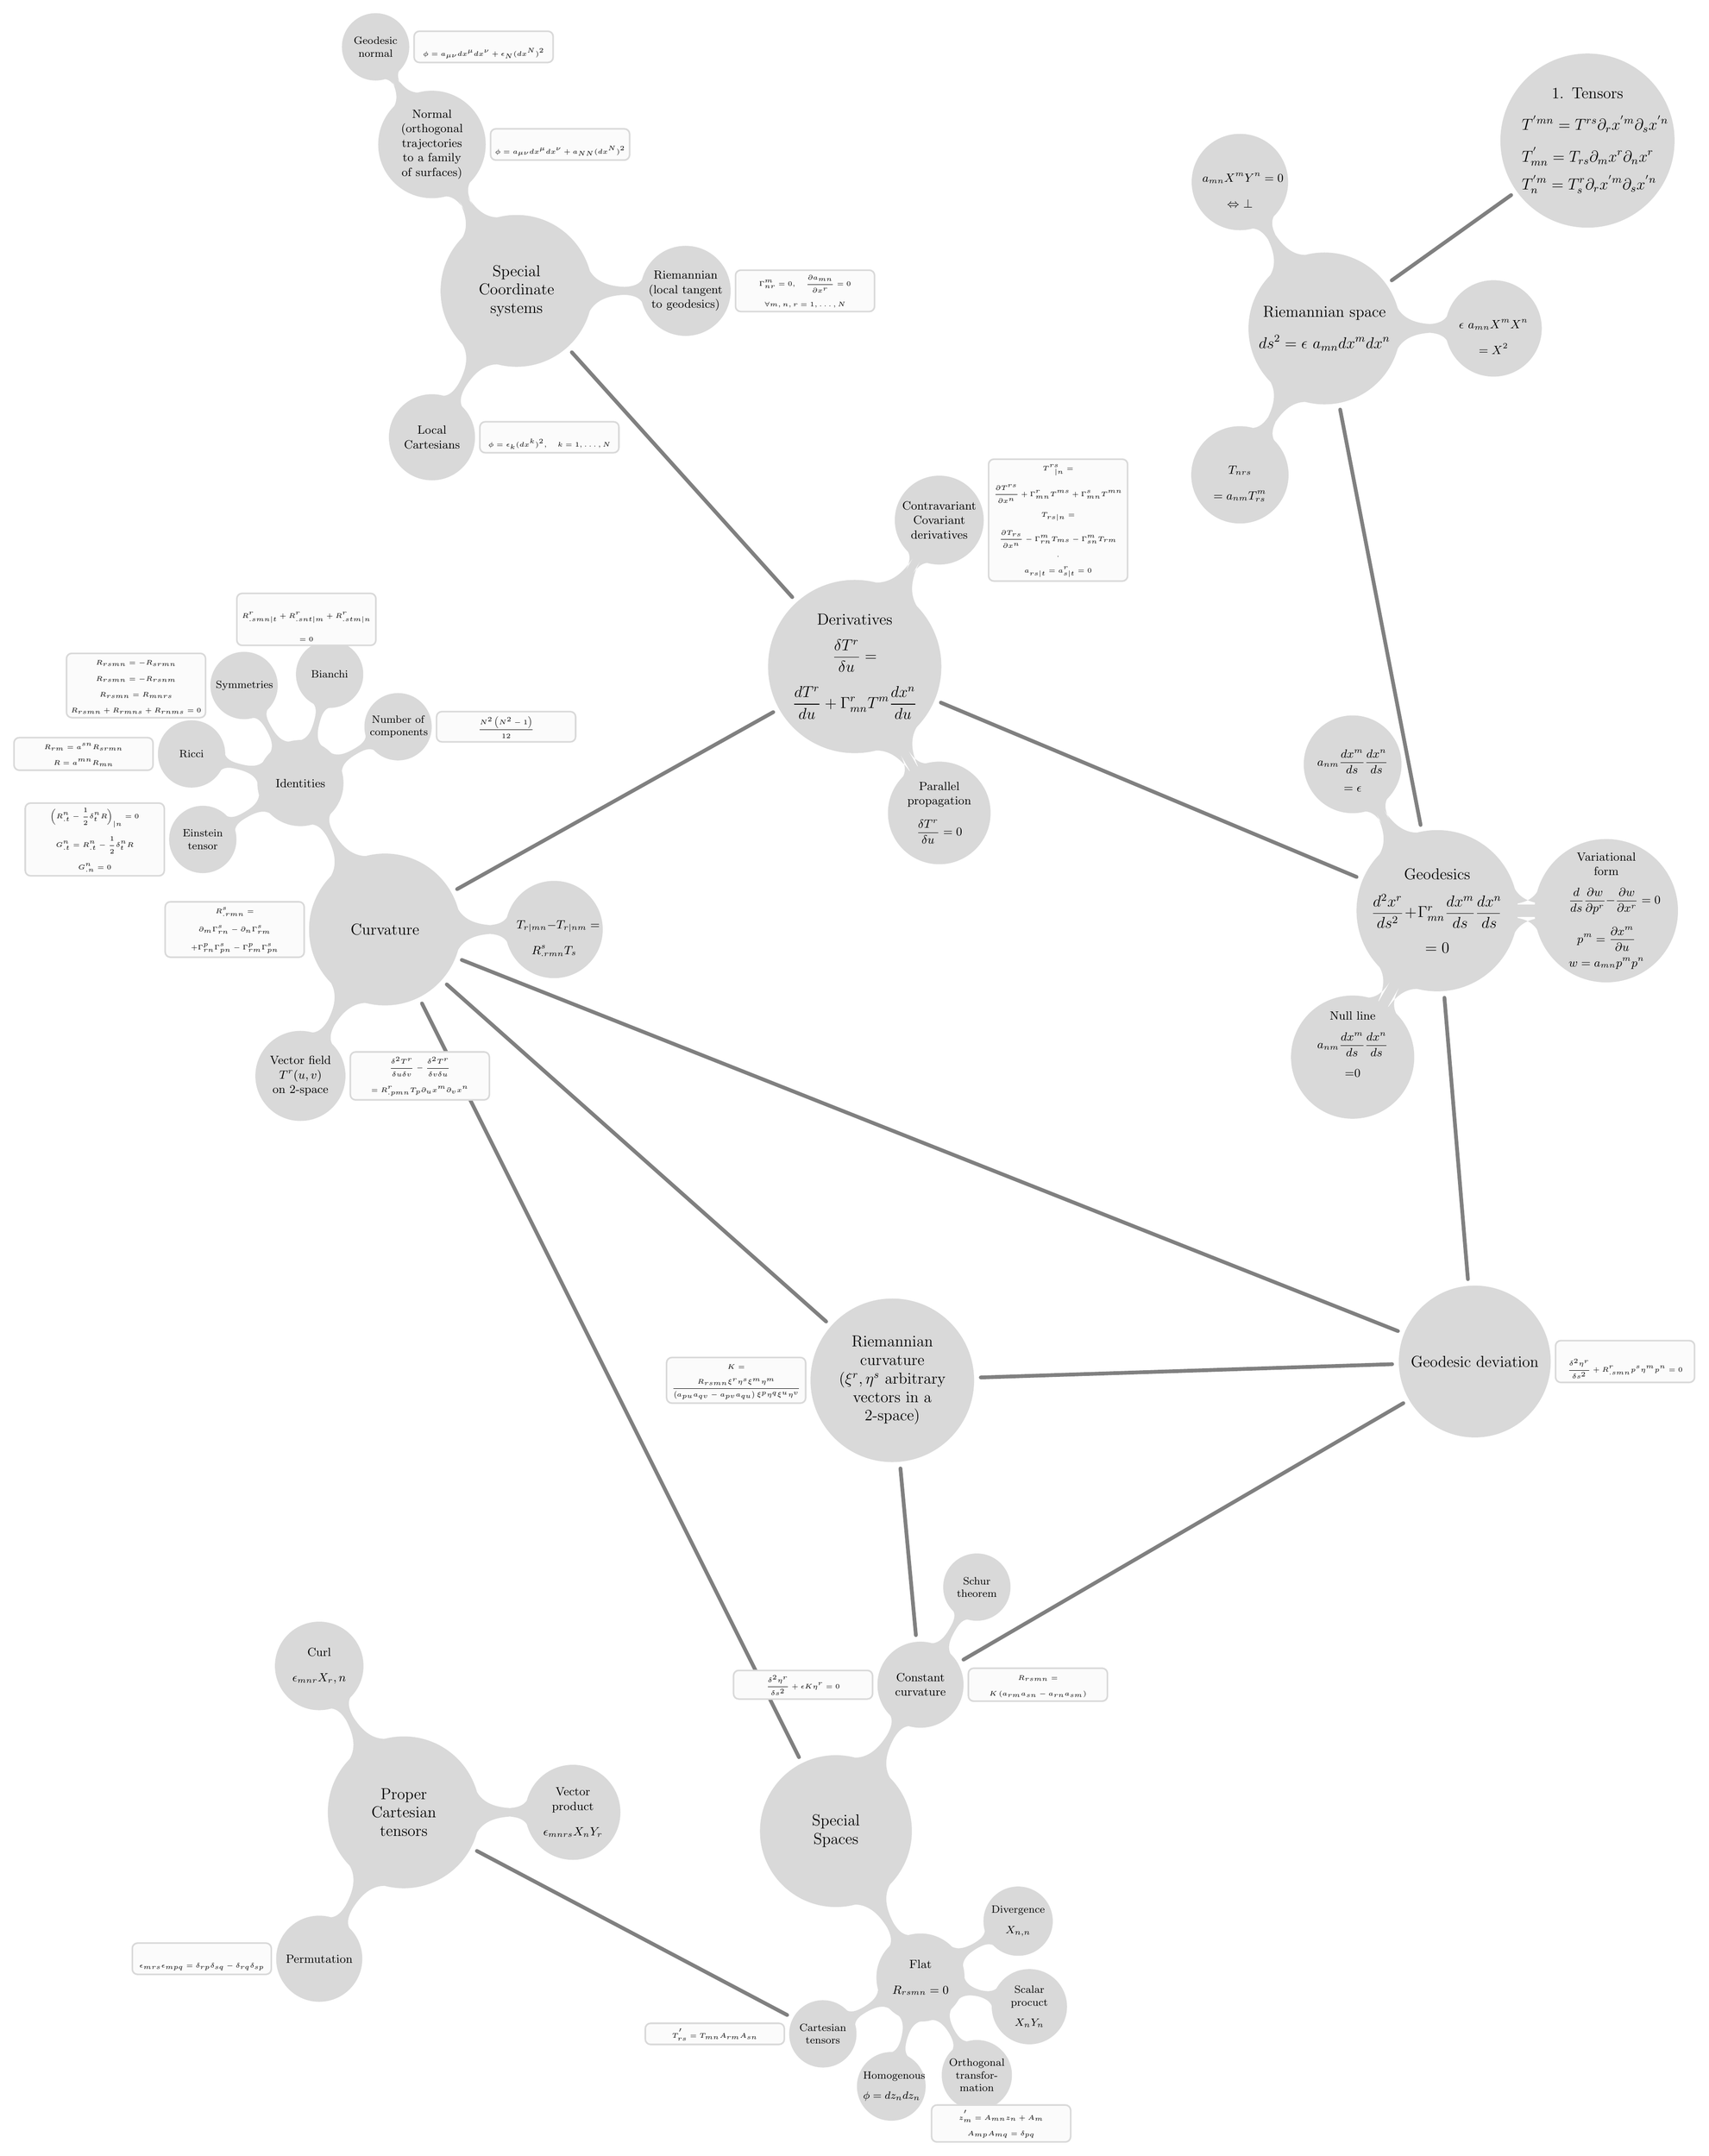
\begin{tikzpicture}[
    mindmap,
    concept color = gray!30,
    every node/.style = {concept},
    grow cyclic,
    minimum size=4cm,
    every annotation/.style={fill=gray!3},
    level 1/.append style = {
        concept color = gray!30,
        %minimum size=4cm,
        level distance = 4.5cm,
        sibling angle = 120
    },
    level 2/.append style = {
        concept color = gray!30,
        %minimum size=4cm,
        level distance = 3cm,
        sibling angle = 45
    }
]
 
\coordinate(N1) at (15.5,26) {} {};
\coordinate(N2) at (8.5,21) {} {};
\coordinate(N3) at (11.5,5.5) {} {};
\coordinate(N4) at (-4,12) {} {} {};
\coordinate(N5) at (-13,22) {} {};
\coordinate(N6) at (-16.5,5) {} {};
\coordinate(N7) at (12.5,-6.5) {} {} {} {};
\coordinate(N8) at (-4.5,-19) {} {} {}{};
\coordinate(N9) at (-16,-18.5) {} {} {} {}{};
%%TENSORS
\node (T1) [concept] at (N1){1. Tensors $$T^{'mn}=T^{rs}\partial_r x^{'m}\partial_s x^{'n}$$
$$T^{'}_{mn}=T_{rs}\partial_m x^{r}\partial_n x^{r}$$
$$T^{'m}_{n}=T^{r}_{s}\partial_r x^{'m}\partial_s x^{'n}$$
};

%%RIEMANNIAN SPACE
 \node (R1) at (N2){Riemannian space $$ds^2=\epsilon \ a_{mn}dx^mdx^n$$}
    child {node {$$T_{nrs}$$ $$=a_{nm}T^m_{rs}$$}
    }
    child {node {$$\epsilon \ a_{mn}X^mX^n$$ $$=X^2$$ }
    }
    child {node {$$    a_{mn}X^mY^n=0$$ $$ \Leftrightarrow \ \perp $$ }
};
 %%GEODESICS
 \node[] (G1) at (N3){Geodesics $$\dv[2]{x^r}{s}+ \Gamma^r_{mn}\dv{x^m}{s}\dv{x^n}{s}$$ $$=0$$}
    
   
    child {node (G1b){Null line$$a_{nm}\dv{x^m}{s}\dv{x^n}{s}$$=0$$ $$}
    }
    child {node(G1c) {Variational form $$\dv{}{s}\pdv{w}{p^r}- \pdv{w}{x^r}=0$$ $$p^m= \pdv{x^m}{u}$$ $$ w= a_{mn}p^mp^n$$}
}
 child {node (G1a){$$a_{nm}\dv{x^m}{s}\dv{x^n}{s}$$$$=\epsilon$$ }
    };




%%DERIVATIVES
\node (D1) at (N4){Derivatives$$\frac{\delta T^r}{\delta u}=$$ $$  \dv{T^r}{u}+\Gamma^r_{mn} T^m\dv{x^n}{u}$$}
    child {node(PP) {Parallel propagation$$\frac{\delta T^r}{\delta u}=0$$}}
    child {node(D2)  {Contravariant \\Covariant\\derivatives }
    };
    \node [annotation,right] at (D2.east){$$ T^{rs}_{\ \ |n}=$$$$\pdv{T^{rs}}{x^n}+\Gamma^r_{mn}T^{ms} +\Gamma^s_{mn}T^{mn} $$ $$  T_{rs|n}=$$$$\pdv{T_{rs}}{x^n}-\Gamma^m_{rn}T_{ms} -\Gamma^m_{sn}T_{rm} $$ $$\mathbf{.}$$ $$a_{rs|t}=a^r_{s|t}=0$$};

%%SPECIAL COORDINATE SYTEMS
\node (SCS1) at (N5){Special \\ Coordinate \\ 
systems}
    child {node(SC1) {Local Cartesians}}
    child {node (SC2) {Riemannian (local tangent to geodesics) }}
    child {node (SC3) {Normal (orthogonal trajectories to a family of surfaces)}child {node(SC4) {Geodesic normal}}
    };
     \node [annotation,right] at (SC1.east){$$ \phi =  \epsilon_{k}(dx^k)^2, \quad k=1,\dots,N$$};
     \node [annotation,right] at (SC2.east){$$\Gamma^m_{nr}=0, \quad \pdv{a_{mn}}{x^r}=0$$$$\forall m,n,r = 1,\dots,N$$};
     \node [annotation,right] at (SC4.east){$$ \phi = a_{\mu\nu}dx^{\mu}dx^{\nu} + \epsilon_N(dx^N)^2$$};
    \node [annotation,right] at (SC3.east){$$ \phi = a_{\mu\nu}dx^{\mu}dx^{\nu} + a_{NN}(dx^N)^2$$};

%%CURVATURE
\node(CR1)  at (N6){Curvature}
    child {node(CR1a) {Vector field $T^r(u,v)$  on 2-space}
    }
    child {node(CR1b) {$$T_{r|mn} - T_{r|nm}= $$$$R^s_{.rmn}T_s$$ }
    }
    child {node(CR1c) {Identities }
    child {node(CR1d) {Number of \\ components}}
    child {node(CR1e) {Bianchi }}
     child {node(CR1f) {Symmetries}}
          child {node(CR1g) {Ricci}}
          child {node(CR1h) {Einstein tensor}}
};


%%GEODESIC DEVIATION
\node(GD1)  at (N7){Geodesic deviation} ;
%%RIEMANNIAN CURVATURE
\node(RC1) at (-3,-7) {Riemannian curvature\\ ($\xi^r,\eta^s$ arbitrary vectors in a \\ 2-space)} ;

%%SPECIAL SPACES
\node (SS) at (N8){Special \\ Spaces}
    child {node(SS1) {Flat$$R_{rsmn}=0$$}
       child {node(SS1c) {Cartesian tensors}}
    child {node(SS1a) {Homogenous $$\phi = dz_ndz_n$$}}
    child {node(SS1b) {Orthogonal transformation}}
    child {node(SS1d) {Scalar procuct$$X_nY_n$$}}
    child {node(SS1e) {Divergence$$X_{n,n}$$}}
    }
    child {node (SS2) {Constant curvature }child {node(SS2a) {Schur theorem}}
    };
    
    %%Proper Cartesian tensors
\node (CT) at (N9){Proper\\ Cartesian \\ tensors}
    child {node(CTa) {Permutation}}
    child {node(CTb) {Vector product$$\epsilon_{mnrs}X_nY_r$$ }}
    child {node(CTc) {Curl$$\epsilon_{mnr}X_r,n$$}
    };
 \node [annotation,right] at (SS2.east){$$R_{rsmn}=$$$$ K\left(a_{rm}a_{sn}-a_{rn}a_{sm}\right)$$};
\node [annotation,left] at (SS2.west){$$\frac{\delta^2\eta^r}{\delta s^2}+\epsilon K\eta^r=0$$}; 
    
\node [annotation,right] at (CR1a.east){$$\frac{\delta^2T^r}{\delta u\delta v}-\frac{\delta^2T^r}{\delta v\delta u}$$$$=R^r_{.pmn}T_p\partial_u x^m\partial_v x^n$$};
\node [annotation,left] at (CR1.west){$$R^s_{.rmn}=$$$$ \partial_m\Gamma^s_{rn}-\partial_n\Gamma^s_{rm}$$$$+\Gamma^p_{rn}\Gamma^s_{pn}-\Gamma^p_{rm}\Gamma^s_{pn}$$};
\node [annotation,left] at (CR1f.west){$$R_{rsmn}=-R_{srmn}$$$$R_{rsmn}=-R_{rsnm}$$$$R_{rsmn}=R_{mnrs}$$$$R_{rsmn}+R_{rmns}+R_{rnms}=0$$};
\node [annotation,above] at (CR1e.north west){$$R^r_{.smn|t}+R^r_{.snt|m}+R^r_{.stm|n}$$$$=0$$};
\node [annotation,right] at (CR1d.east){$$\frac{ N^2\left(N^2-1\right)}{12}$$ };
\node [annotation,left] at (CR1g.west){$$R_{rm}= a^{sn}R_{srmn}$$$$R=a^{mn}R_{mn}$$ };
\node [annotation,left] at (CR1h.west){$$\left( R^n_{.t} - \frac{1}{2}\delta^n_t R \right)_{|n}=0$$ $$G^n_{.t} = R^n_{.t} - \frac{1}{2}\delta^n_t R $$$$G^n_{.n}=0$$ };
\node [annotation,right] at (GD1.east){$$\frac{\delta^2\eta^r}{\delta s^2}+R^r_{.smn}p^s\eta^m p^n=0$$};
\node [annotation,left] at (RC1.west){$$K = $$ $$\frac{R_{rsmn}\xi^r\eta^s \xi^m\eta^m}{\left(a_{pu}a_{qv}-a_{pv}a_{qu}\right)\xi^p\eta^q \xi^u\eta^v}$$};
\node [annotation,below] at (SS1b.south east){$$z^{'}_{m}=A_{mn}z_n+A_m $$ $$A_{mp}A_{mq}= \delta_{pq}$$};
\node [annotation,left] at (SS1c.west){$$T^{'}_{rs}= T_{mn}A_{rm}A_{sn}$$ };
\node [annotation,left] at (CTa.west){$$\epsilon_{mrs}\epsilon_{mpq} = \delta_{rp}\delta_{sq}-\delta_{rq}\delta_{sp}$$ };


\begin{pgfonlayer}{background}
    \draw [concept connection]  (D1) edge (SCS1);
    \draw [concept connection]  (T1) edge (R1);
    \draw [concept connection]  (R1) edge (G1);
    \draw [concept connection]  (G1) edge (D1);
    \draw [concept connection]  (D1) edge (CR1);
    \draw [concept connection]  (CR1) edge (GD1);
     \draw [concept connection]  (G1) edge (GD1);
     \draw [concept connection]  (CR1) edge (RC1);
     \draw [concept connection]  (RC1) edge (GD1);
      \draw [concept connection]  (CR1) edge (SS);
      \draw [concept connection]  (RC1) edge (SS2);
      \draw [concept connection]  (GD1) edge (SS2);
      \draw [concept connection]  (SS1c) edge (CT);
  \end{pgfonlayer}
\end{tikzpicture}
 
\end{document}